\chapter{SOFT VOXEL ACTUATORS: HYDROGEL BUILDING BLOCKS FOR BOTTOM UP ASSEMBLY OF SOFT ROBOTS}
Although progress has been made in automated manufacturing of soft robots, there is still some challenges remained. For example, 3D printing electronic circuits require soft electronics materials compatible with 3D printing techniques that can be simultaneously printed with the main body of the robot. Bottom up manufacturing methods in which a building block is used to assemble more complex structure seem more promising. 

what is heterogeneity?
detailed literature survey
soft voxel actuators
\section{Section1}
Two types of SVAs have been realized and are described herein: one without an embedded heater (referred to as SVA-I), and one with an embedded heater (referred to as SVA-II), as shown in \subfigref{fig:1}{B}. Various combinations of SVA-I and SVA-II can be used for designing and fabricating heterogeneous assemblies. One possible combination, shown in \subfigref{fig:1}{B(i)}, uses SVA-I to create pre-programmed voxel assemblies. Based on the specific arrangement of SVA-I consisting of different swelling properties (mainly volume change ratio and rate), complex deformations can be demonstrated. These SVA assemblies deform in response to regular and repeated homogeneous temperature changes (such as the bulk heating and cooling of a water reservoir), generating motions without the need for an on-board energy source. It should be noted that hydrogels expand and contract based on the diffusion of water into and out of their structure when the temperature is passed their critical transition temperature which is around 32\textsuperscript{o} C in case of PNIPAAm hydrogels. Therefore, all our experiments are performed in a water bath. Another combination of SVAs shown in \subfigref{fig:1}{B(ii)}, uses thick film surface mount (SMD) resistive elements with a resistance of 10 ohms as Joule heaters in SVA-II units to create time-varying and inhomogeneous temperature fields, resulting in on-demand dynamic deformations and real-time reconfigurability. Details of the Joule heater elements are presented in the Supporting Information.\\ 
\section{Section2}

\begin{figure}[t]
\centering
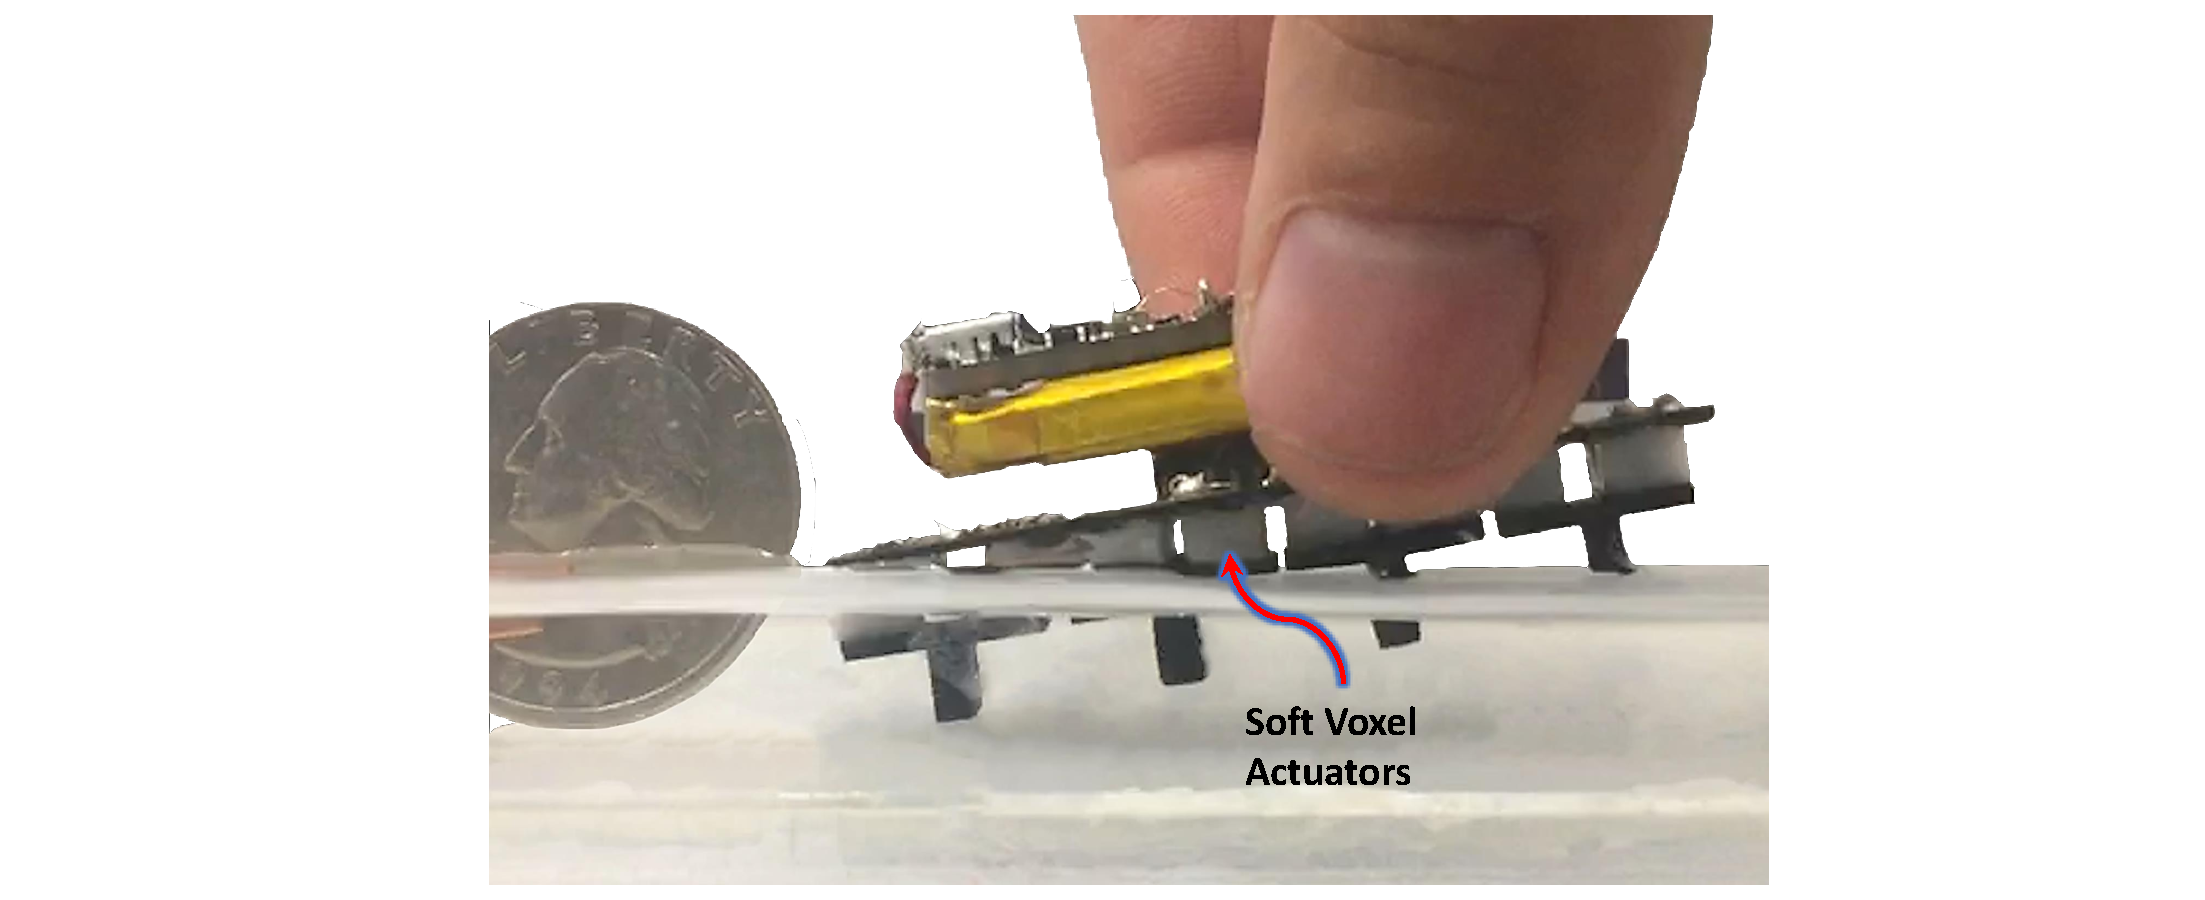
\includegraphics[width=0.48\textwidth]{Images/chap3/Fig1.pdf}
    \caption{Soft Voxel Actuators (SVAs) are individually addressable hydrogel-based actuators that can aid in miniaturizing and cutting the tether from soft robots. 
    % A) A hyper-redundant miniature manipulator using 16 SVAs. B) 
    An exemplary untethered miniature underwater walking robot using 8 SVAs is shown which weighs only 20\,g including battery and electronics.}
    \label{fig:concept}
\end{figure}
\begin{figure*}[th]
      \centering
      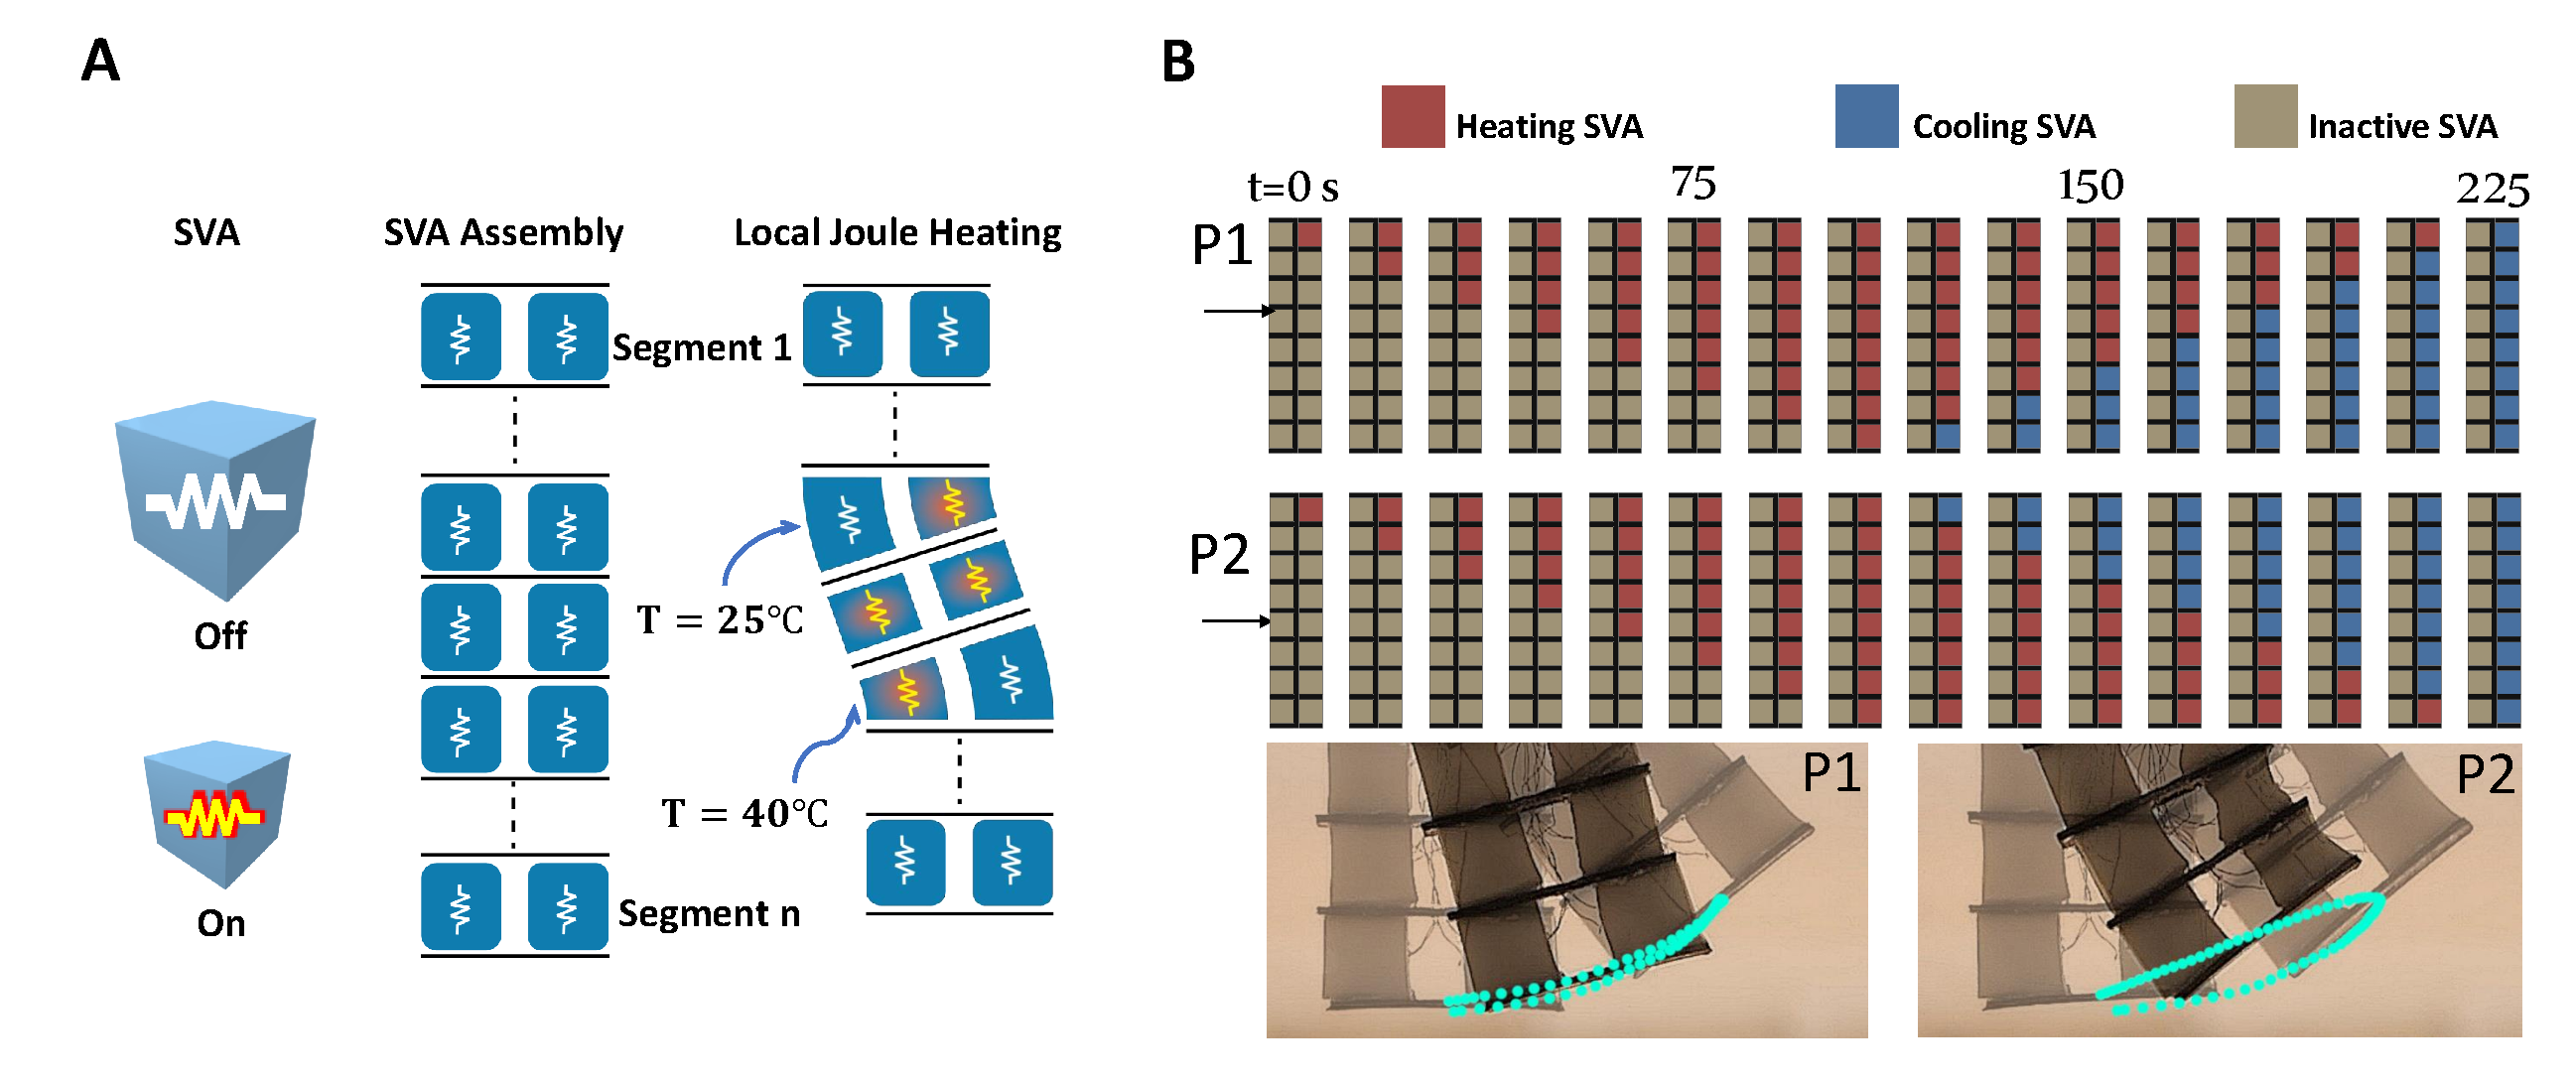
\includegraphics[scale=0.4]{Images/chap3/Fig2.pdf}
      \caption{A) On and off states of a SVA is shown on the left column. Schematic of an assembly of SVAs is shown on the middle column. Activation of SVAs results in local increase in the temperature which leads to deformations that control the overall motion of the manipulator (right column). B) Sequentially activating SVAs 1 through 8 according to the patterns labeled P1 and P2 results in different trajectories followed by the tip of the manipulator (shown in cyan at the bottom). For details, see Movie S1.}
      \label{fig:treajectory}
   \end{figure*}